\documentclass{sigchi}

% Use this command to override the default ACM copyright statement (e.g. for preprints). 
% Consult the conference website for the camera-ready copyright statement.


%% EXAMPLE BEGIN -- HOW TO OVERRIDE THE DEFAULT COPYRIGHT STRIP -- (July 22, 2013 - Paul Baumann)
% \toappear{Permission to make digital or hard copies of all or part of this work for personal or classroom use is 	granted without fee provided that copies are not made or distributed for profit or commercial advantage and that copies bear this notice and the full citation on the first page. Copyrights for components of this work owned by others than ACM must be honored. Abstracting with credit is permitted. To copy otherwise, or republish, to post on servers or to redistribute to lists, requires prior specific permission and/or a fee. Request permissions from permissions@acm.org. \\
% {\emph{CHI'14}}, April 26--May 1, 2014, Toronto, Canada. \\
% Copyright \copyright~2014 ACM ISBN/14/04...\$15.00. \\
% DOI string from ACM form confirmation}
%% EXAMPLE END -- HOW TO OVERRIDE THE DEFAULT COPYRIGHT STRIP -- (July 22, 2013 - Paul Baumann)


% Arabic page numbers for submission. 
% Remove this line to eliminate page numbers for the camera ready copy
\pagenumbering{arabic}


% Load basic packages
\usepackage{balance}  % to better equalize the last page
\usepackage{graphics} % for EPS, load graphicx instead
\usepackage{times}    % comment if you want LaTeX's default font
\usepackage{url}      % llt: nicely formatted URLs
\usepackage{color}


% llt: Define a global style for URLs, rather that the default one
\makeatletter
\def\url@leostyle{%
  \@ifundefined{selectfont}{\def\UrlFont{\sf}}{\def\UrlFont{\small\bf\ttfamily}}}
\makeatother
\urlstyle{leo}


% To make various LaTeX processors do the right thing with page size.
\def\pprw{210mm}
\def\pprh{297mm}
\special{papersize=\pprw,\pprh}
\setlength{\paperwidth}{\pprw}
\setlength{\paperheight}{\pprh}
\setlength{\pdfpagewidth}{\pprw}
\setlength{\pdfpageheight}{\pprh}

% Make sure hyperref comes last of your loaded packages, 
% to give it a fighting chance of not being over-written, 
% since its job is to redefine many LaTeX commands.
\usepackage[pdftex]{hyperref}
\hypersetup{
pdftitle={Supporting public deliberation through spatially enhanced dialogues},
pdfauthor={LaTeX},
bookmarksnumbered,
pdfstartview={FitH},
colorlinks,
citecolor=black,
filecolor=black,
linkcolor=black,
urlcolor=black,
breaklinks=true,
}

% create a shortcut to typeset table headings
\newcommand\tabhead[1]{\small\textbf{#1}}


% End of preamble. Here it comes the document.
\begin{document}

\title{Supporting public deliberation\\through spatially enhanced dialogues}
\subtitle{Master thesis}

\numberofauthors{1}
\author{
  \alignauthor Gerald Pape\\
    \affaddr{Institute for Geoinformatics}\\
    \email{g.pape@uni-muenster.de}\\
%   \alignauthor 2nd Author Name\\
%     \affaddr{Affiliation}\\
%     \affaddr{Address}\\
%     \email{e-mail address}\\
%     \affaddr{Optional phone number}    
%   \alignauthor 3rd Author Name\\
%     \affaddr{Affiliation}\\
%     \affaddr{Address}\\
%     \email{e-mail address}\\
%     \affaddr{Optional phone number}
}

\maketitle

\begin{abstract}
swaghetti yolonaise
\end{abstract}

% \keywords{
% 	Guides; instructions; author's kit; conference publications;
% 	keywords should be separated by a semi-colon.
% 	\textcolor{red}{Mandatory section to be included in your final version.}
% }

% \category{H.5.m.}{Information Interfaces and Presentation (e.g. HCI)}{Miscellaneous}

% See: \url{http://www.acm.org/about/class/1998/}
% for more information and the full list of ACM classifiers
% and descriptors. 
% \textcolor{red}{Mandatory section to be included in your
% final version. On the submission page only the classifiers'
% letter-number combination will need to be entered.}

\section{Introduction}

Interactivity and collaboration are core characteristics of Web 2.0 applications. This holds 


\section{Related Work}

\subsubsection{Argumentation mapping}
Rinner\cite{Rinner_ArgumentationMaps}\dots

Existing implementations\dots

Evaluation\dots
\subsubsection{Public deliberation and eParticipation}


\section{Approach}

\subsubsection{DialogMap}

In order to test the initial idea of supporting public deliberation through spatially enhanced dialogues, a working prototype had to be developed. 

Input and opinions from potential users with specific use cast in the future.




\subsubsection{Design decisions} % and features

As seen in X,Y and Z, important aspects of A are\dots

\begin{itemize}
\item Map view with sidebar on right hand side
\item Two way highlighting between contributions in sidebar and features on map
\item Creation of Topic with \begin{itemize}
    \item Title
    \item Category/ies \begin{itemize}
        \item in this specific case for two dimensions \begin{itemize}
            \item Color
            \item Icon
            \end{itemize}
        \end{itemize}
    \item Tags
    \item Time limit
    \item Image
    \item Special Description field which allows to create \begin{itemize}
        \item Points and Polygons
        \item References to existing Points and Polygons
        \item Hyperlinks
        \end{itemize}
    \end{itemize}
\item Sorting
\item Filter \begin{itemize}
    \item Fulltext
    \item Categories
    \item Tags
    \item Time
\end{itemize}
\item Favorites
\item Register/Sign in \begin{itemize}
    \item with Google,Facebook, Twitter
    \end{itemize}
\end{itemize}


\subsubsection{Implementation}
\textit{DialogMap} has been implemented as a single-page web application using AngularJS\footnote{\url{http://angularjs.org/}} and Ruby on Rails\footnote{\url{http://rubyonrails.org/}}. The single-page structure was chosen in order to provide the user with a clear navigation between the overview and contribution answers. This also allows for a seamless browsing experience without full reloads of the page. AngularJS is a JavaScript framework with features like templating, two-way binding and DOM manipulation. It follows the model-view-controller pattern in order to bring server side paradigms to client-side development. AngularJS was chosen because of its popularity, extensibility and high number of available libraries. It also enables to wrap existing JavaScript libraries to be used in AngularJS context.\\
The mapping library Leaflet\footnote{\url{http://leafletjs.com/}} serves as base for displaying base maps and geospatial data. The user-facing web page was developed using tools like CoffeeScript\footnote{\url{http://coffeescript.org/}}, Haml\footnote{\url{http://haml.info/}} and Sass\footnote{\url{http://sass-lang.com/}} to speed up the development. The web page was developed with all major browsers in mind.\\
On the server side, components were developed using the Ruby on Rails framework with PostgreSQL\footnote{\url{http://www.postgresql.org/}}/PostGIS\footnote{\url{http://postgis.net/}} as data storage. Ruby on Rails, originally a full-stack model-view-controller web framework, is used as a JSON serving application logic. It was chosen because of its maturity and high number of available libraries. Front- and backend of the application communicate in REST\footnote{Representational State Transfer}-API\footnote{Application programming interface} like manner. This allows for easily replaceable front- and backend application stacks.\\
Figure \ref{fig:screenshot} shows the web page with an active two way highlight.\\
Without the extensive use of open source software and code, development would have taken much longer. It is planned to release the source code through github\footnote{\url{https://github.com/ubergesundheit/dialogmap}}.

\begin{figure}[!h]
    \centering
    \includegraphics[width=0.9\columnwidth]{screenshot}
    \caption{Screenshot of the \textit{DialogMap} with active highlight of a contribution and spatial feature.}
    \label{fig:screenshot}
\end{figure}


\section{Evaluation}

Interviews

Utility evaluation

Types of questions

Results

\section{Conclusion}

This work discusses the implementation and pre-evaluation of an application to support public deliberation through spatially enhanced dialogues.

\subsubsection{Future Work}
Pick up shortcomings emerged during evaluation. Point to solutions...

Legal implications of running such a website have to be explored.

% \section{Figure and Table Example}

% \begin{figure}[!h]
% \centering
% 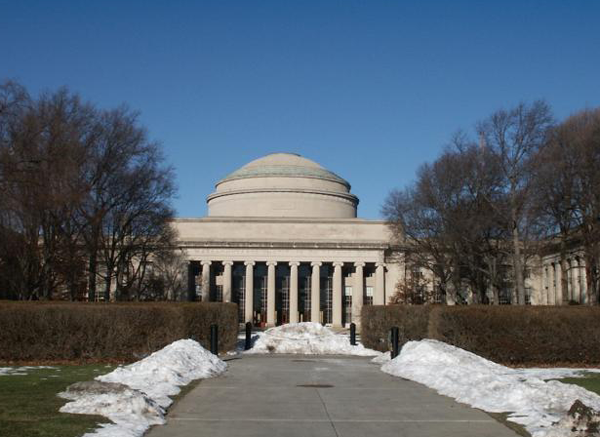
\includegraphics[width=0.9\columnwidth]{Figure1}
% \caption{With Caption Below, be sure to have a good resolution image
%   (see item D within the preparation instructions).}
% \label{fig:figure1}
% \end{figure}

% \begin{table}
%   \centering
%   \begin{tabular}{|c|c|c|}
%     \hline
%     \tabhead{Objects} &
%     \multicolumn{1}{|p{0.3\columnwidth}|}{\centering\tabhead{Caption --- pre-2002}} &
%     \multicolumn{1}{|p{0.4\columnwidth}|}{\centering\tabhead{Caption --- 2003 and afterwards}} \\
%     \hline
%     Tables & Above & Below \\
%     \hline
%     Figures & Below & Below \\
%     \hline
%   \end{tabular}
%   \caption{Table captions should be placed below the table.}
%   \label{tab:table1}
% \end{table}



% Balancing columns in a ref list is a bit of a pain because you
% either use a hack like flushend or balance, or manually insert
% a column break.  http://www.tex.ac.uk/cgi-bin/texfaq2html?label=balance
% multicols doesn't work because we're already in two-column mode,
% and flushend isn't awesome, so I choose balance.  See this
% for more info: http://cs.brown.edu/system/software/latex/doc/balance.pdf
%
% Note that in a perfect world balance wants to be in the first
% column of the last page.
%
% If balance doesn't work for you, you can remove that and
% hard-code a column break into the bbl file right before you
% submit:
%
% http://stackoverflow.com/questions/2149854/how-to-manually-equalize-columns-
% in-an-ieee-paper-if-using-bibtex
%
% Or, just remove \balance and give up on balancing the last page.
%
\newpage
\balance

% REFERENCES FORMAT
% References must be the same font size as other body text.

\bibliographystyle{acm-sigchi}
\bibliography{masterthesis-pape}
\end{document}
